\documentclass[11pt,a4paper,twoside]{book}
\usepackage[]{graphicx}\usepackage[]{color}
%% maxwidth is the original width if it is less than linewidth
%% otherwise use linewidth (to make sure the graphics do not exceed the margin)
\makeatletter
\def\maxwidth{ %
  \ifdim\Gin@nat@width>\linewidth
    \linewidth
  \else
    \Gin@nat@width
  \fi
}
\makeatother

\definecolor{fgcolor}{rgb}{0.345, 0.345, 0.345}
\newcommand{\hlnum}[1]{\textcolor[rgb]{0.686,0.059,0.569}{#1}}%
\newcommand{\hlstr}[1]{\textcolor[rgb]{0.192,0.494,0.8}{#1}}%
\newcommand{\hlcom}[1]{\textcolor[rgb]{0.678,0.584,0.686}{\textit{#1}}}%
\newcommand{\hlopt}[1]{\textcolor[rgb]{0,0,0}{#1}}%
\newcommand{\hlstd}[1]{\textcolor[rgb]{0.345,0.345,0.345}{#1}}%
\newcommand{\hlkwa}[1]{\textcolor[rgb]{0.161,0.373,0.58}{\textbf{#1}}}%
\newcommand{\hlkwb}[1]{\textcolor[rgb]{0.69,0.353,0.396}{#1}}%
\newcommand{\hlkwc}[1]{\textcolor[rgb]{0.333,0.667,0.333}{#1}}%
\newcommand{\hlkwd}[1]{\textcolor[rgb]{0.737,0.353,0.396}{\textbf{#1}}}%
\let\hlipl\hlkwb

\usepackage{framed}
\makeatletter
\newenvironment{kframe}{%
 \def\at@end@of@kframe{}%
 \ifinner\ifhmode%
  \def\at@end@of@kframe{\end{minipage}}%
  \begin{minipage}{\columnwidth}%
 \fi\fi%
 \def\FrameCommand##1{\hskip\@totalleftmargin \hskip-\fboxsep
 \colorbox{shadecolor}{##1}\hskip-\fboxsep
     % There is no \\@totalrightmargin, so:
     \hskip-\linewidth \hskip-\@totalleftmargin \hskip\columnwidth}%
 \MakeFramed {\advance\hsize-\width
   \@totalleftmargin\z@ \linewidth\hsize
   \@setminipage}}%
 {\par\unskip\endMakeFramed%
 \at@end@of@kframe}
\makeatother

\definecolor{shadecolor}{rgb}{.97, .97, .97}
\definecolor{messagecolor}{rgb}{0, 0, 0}
\definecolor{warningcolor}{rgb}{1, 0, 1}
\definecolor{errorcolor}{rgb}{1, 0, 0}
\newenvironment{knitrout}{}{} % an empty environment to be redefined in TeX

\usepackage{alltt}
\newcommand{\SweaveOpts}[1]{}  % do not interfere with LaTeX
\newcommand{\SweaveInput}[1]{} % because they are not real TeX commands
\newcommand{\Sexpr}[1]{}       % will only be parsed by R


% We load package by package and set package relevant parameters.
% Topics are summarized later
%%%%%%%%%%%%%%%%%%%%%%%%%%%%%%%%%%%%%%%%%%%%%%%%%%%%%%%%%%%%%%%%%%%%%%%%
% helping packages
\usepackage{ifthen}
\usepackage{calc}

\usepackage[T1]{fontenc}       % provides fonts having  accented characters 
\usepackage[latin1]{inputenc}  % allows the user to input accented characters directly from the keyboard

%%%%%%%%%%%%%%%%%%%%%%%%%%%%%%%%%%%%%%%%%%%%%%%%%%%%%%%%%%%%%%%%%%%%%%%%

\renewcommand{\baselinestretch}{1.2}
\renewcommand{\textfraction}{0}%0.2     % placement of figures
\renewcommand{\topfraction}{1}%.3
\renewcommand{\bottomfraction}{1}%.3
\renewcommand{\floatpagefraction}{1}%.3
\setcounter{bottomnumber}{3}%1

\textwidth6.3in
\textheight9.7in
\topmargin-45pt
\oddsidemargin-.15in
\evensidemargin.15in
\headsep30pt
\headheight15pt
%\footskip20pt


%%%%%%%%%%%%%%%%%%%%%%%%%%%%%%%%%%%%%%%%%%%%%%%%%%%%%%%%%%%%%%%%%%%%%%%%

\usepackage[dvipsnames]{xcolor}
\definecolor{fgcolor}{rgb}{0.345, 0.345, 0.345}
\definecolor{shadecolor}{rgb}{.97, .97, .97}
\definecolor{messagecolor}{rgb}{0, 0, 0}
\definecolor{warningcolor}{rgb}{1, 0, 1}
\definecolor{errorcolor}{rgb}{1, 0, 0}
\definecolor{DarkBlue}{rgb}{0,0,0.5451}
\definecolor{DarkGreen}{rgb}{0,0.39216,0}
\definecolor{LightYellow}{rgb}{1,1,.8}
\definecolor{orange}{rgb}{.9,0.3445,0}



%%%%%%%%%%%%%%%%%%%%%%%%%%%%%%%%%%%%%%%%%%%%%%%%%%%%%%%%%%%%%%%%%%%%%%%%
\usepackage{afterpage}
\usepackage{natbib}
\usepackage{upquote}

\usepackage[english]{babel}

%%%%%%%%%%%%%%%%%%%%%%%%%%%%%%%%%%%%%%%%%%%%%%%%%%%%%%%%%%%%%%%%%%%%%%%%%%%%%%%
%% maxwidth is the original width if it is less than linewidth
%% otherwise use linewidth (to make sure the graphics do not exceed the margin)
\makeatletter
\def\maxwidth{ %
  \ifdim\Gin@nat@width>\linewidth
    \linewidth
  \else
    \Gin@nat@width
  \fi
}
\makeatother

%%%%%%%%%%%%%%%%%%%%%%%%%%%%%%%%%%%%%%%%%%%%%%%%%%%%%%%%%%%%%%%%%%%%%%%%%%%%%%%%%%%%%%%%%%%%%%%%%%%%%%%%%%%%
% from fancyvrb
\usepackage{fancyhdr}
\usepackage{fancyvrb}
\DefineVerbatimEnvironment{Rcode}{Verbatim}{xleftmargin=2em,fontshape=sl,formatcom=\color{DarkGreen}}
\fvset{listparameters={\setlength{\topsep}{0pt}}}

%%%%%%%%%%%%%%%%%%%%%%%%%%%%%%%%%%%%%%%%%%%%%%%%%%%%%%%%%%%%%%%%%%%%%%%%%%%%%%%%%%%%%%%%%%%%%%%%%%%%%%%%%%%%%
\usepackage{float}
\usepackage{graphicx}
\usepackage[margin=2em,labelfont=bf]{caption}


%%%%%%%%%%%%%%%%%%%%%%%%%%%%%%%%%%%%%%%%%%%%%%%%%%%%%%%%%%%%%%%%%%%%%%%%
\usepackage[pdftex,plainpages=false,pdfpagelabels,pagebackref=true,colorlinks=true,pdfpagemode=UseOutlines]{hyperref}


%%%%%%%%
\usepackage{tabularx}
%%%%%%%%

%%%%%%%%%%%%%%%%%%%%%%%%%%%%%%%%%%%%%%%%%%%%%%%%%%%%%%%%%%%%%%%%%%%%%%%%
% now math stuff and other details...
\usepackage{amsmath,amsthm,amssymb}

\newtheorem{pro}{Property}[chapter]
\theoremstyle{definition}
\newtheorem{des}{Definition}[chapter]
\newtheorem{bsp}{Example}[chapter]
\newtheorem{rem}{Remark}[chapter]

\newcommand*\widebar[1]{%
  \vbox{%
    \hrule height 0.5pt%     % Line above with certain width
    \kern0.5ex%             % Distance between line and content
    \hbox{%
      \kern-0.1em%           % Distance between content and left side of box, negative values for lines shorter than content
      \ifmmode#1\else\ensuremath{#1}\fi%  % The content, typeset in dependence of mode
      \kern-0.1em%      % Distance between content and left side of box, negative values for lines shorter than content
    }% end of hbox
  }% end of vbox
}
\def\ds{\displaystyle}

\newcommand{\rr}[1]{{\ttfamily\slshape\color{DarkGreen} #1}}

\makeatletter


% clever trick to circumvent potential redefines after loading packages:
% \providecommand{\something}{}  % if it does not exist, it creates it.
%      has same syntax as \newcommand
% \renewcommand{\something}{....}
% TUGboat 29(2)


\makeatletter
%umdefinierung exisitierender befehle
\let\oldH\H
\let\oldL\L
\let\oldO\H
\let\oldS\S
\let\olda\a
\let\oldb\b
\let\oldc\c
\let\oldd\d
\let\oldk\k
\let\oldv\v
\let\oldl\l
\let\oldt\t
\let\oldu\u
\let\oldIJ\IJ
\let\oldP\P
\let\P\relax
\let\oldnorm\|

%\DefineVerbatimEnvironment{CodeInput}{Verbatim}{fontshape=sl}
%\DefineVerbatimEnvironment{CodeOutput}{Verbatim}{}

% some classical environments, up-right, with chapter numbering.
\theoremstyle{definition}
\newtheorem{definition}{Definition}[chapter]
\newtheorem{example}{Example}[chapter]
\newtheorem{remark}{Remark}[chapter]
\newtheorem{theorem}{Theorem}[chapter]



\renewcommand{\|}{|\!|}         % closer norm
\newcommand{\T}{{}^{\top}}
\newcommand\code[1]{{\tt#1}}



\newcounter{algo}
\newenvironment{algorithm}{%
  \begin{list}{
      (\arabic{algo})
    }{
      \usecounter{algo}
    }%
}{
  \end{list}
}

% some text abbreviation
\newcommand{\GLS}{\text{GLS}}
\newcommand{\RR}{\text{RR}}
\newcommand{\OR}{\text{OR}}
\newcommand{\WLS}{\text{WLS}}
\newcommand{\MLE}{\text{MLE}}
\newcommand{\OLS}{\text{OLS}}
\newcommand{\MAE}{\text{MAE}}
\newcommand{\MAD}{\text{MAD}}
\newcommand{\RMSE}{\text{RMSE}}
\newcommand{\SVAR}{\text{svar}} %silvanos new commands
\newcommand{\EVAR}{\text{evar}}
\newcommand{\LMG}{\text{LMG}}
\newcommand{\Rtwo}{\text{R}^2}



\newcommand{\ii}{\text{\i}}

\newcommand{\Bin}{\cB\mathit{\!i\!n}}
\newcommand{\Beta}{\cB\mathit{\!e\!t\!a}}
\newcommand{\Pois}{\cP\mathit{\!o\!i\!s\!s\!o\!n}}
\newcommand{\Exp}{\cE\mathit{\!x\!p}}


\DeclareMathOperator*{\argmin}{argmin}
\DeclareMathOperator*{\argmax}{argmax}
\DeclareMathOperator{\diag}{diag}
\DeclareMathOperator{\diam}{diam}
\DeclareMathOperator{\card}{card}
\DeclareMathOperator{\cov}{Cov}                   
\DeclareMathOperator{\corr}{Corr}                 
\DeclareMathOperator{\var}{Var}                   
\DeclareMathOperator{\trace}{tr}                  
\DeclareMathOperator{\E}{E}                       
\DeclareMathOperator{\P}{P}                       
\DeclareMathOperator{\pred}{p}
\DeclareMathOperator{\vect}{vec}                  
\DeclareMathOperator{\vech}{vech}                 
\DeclareMathOperator{\rank}{rank}                 
\DeclareMathOperator{\e}{e}                       
%\DeclareMathOperator{\cv}{CV}                     
\DeclareMathOperator{\GCV}{GCV}                     
\DeclareMathOperator{\CV}{CV}                     
\DeclareMathOperator{\BLUP}{BLUP}                 
\DeclareMathOperator{\MSE}{MSE}                   
\DeclareMathOperator{\MS}{MS}                   
\DeclareMathOperator{\df}{df}                   
\DeclareMathOperator{\bias}{bias}                   
\DeclareMathOperator{\eig}{eig}                   
\DeclareMathOperator{\Prec}{Prec}
\DeclareMathOperator{\mode}{mode}
\renewcommand{\SS}{\text{SS}}
\renewcommand{\d}{\mathsf{\,d}}

\def\arctanh{\qopname\relax o{arctanh}}  % as in amsopn
\newcommand{\bigo}{\cO}
\newcommand{\lito}{\text{\scriptsize{$\cO$}}}
\newcommand{\cdfPhi}{\itPhi}
\newcommand{\ml}{_\text{ML}}

\newcommand*{\stack@relbin}[3][]{%
  \mathop{#3}\limits
  \toks@{#1}%
  \edef\reserved@a{\the\toks@}%
  \ifx\reserved@a\@empty\else_{#1}\fi
  \toks@{#2}%
  \edef\reserved@a{\the\toks@}%
  \ifx\reserved@a\@empty\else^{#2}\fi
  \egroup
}%
\renewcommand*{\stackrel}{\mathrel\bgroup\stack@relbin}
\newcommand*{\stackbin}{\mathbin\bgroup\stack@relbin}
\newcommand{\simiid}{\stackrel[]{\text{iid}}{\sim}}

% Kalligraphischer Schriftsatz
\newcommand{\cA}{{\cal{A}}}
\newcommand{\cB}{{\cal{B}}} 
\newcommand{\cC}{{\cal{C}}}
\newcommand{\cD}{{\cal{D}}} 
\newcommand{\cE}{{\cal{E}}}
\newcommand{\cF}{{\cal{F}}}
\newcommand{\cG}{{\cal{G}}}
\newcommand{\cH}{{\cal{H}}}
\newcommand{\cI}{{\cal{I}}}
\newcommand{\cJ}{{\cal{J}}}
\newcommand{\cK}{{\cal{K}}}
\newcommand{\cL}{{\cal{L}}}
\newcommand{\cM}{{\cal{M}}} 
\newcommand{\cN}{{\cal{N}}}
\newcommand{\cO}{{\cal{O}}} 
\newcommand{\cP}{{\cal{P}}}
\newcommand{\cQ}{{\cal{Q}}} 
\newcommand{\cR}{{\cal{R}}} 
\newcommand{\cS}{{\cal{S}}} 
\newcommand{\cT}{{\cal{T}}}
\newcommand{\cU}{{\cal{U}}}
\newcommand{\cV}{{\cal{V}}}
\newcommand{\cW}{{\cal{W}}}
\newcommand{\cX}{{\cal{X}}} 
\newcommand{\cY}{{\cal{Y}}}
\newcommand{\cZ}{{\cal{Z}}} 


\newcommand{\IA}{{\mathbb{A}}}
\newcommand{\IB}{{\mathbb{B}}}
\newcommand{\IC}{{\mathbb{C}}}
\newcommand{\ID}{{\mathbb{D}}}
\newcommand{\IE}{{\mathbb{E}}}
\newcommand{\IF}{{\mathbb{F}}}
\newcommand{\IG}{{\mathbb{G}}}
\newcommand{\IH}{{\mathbb{H}}}
\newcommand{\II}{{\mathbb{I}}}
%\newcommand{\IJ}{{\mathbb{J}}}
\newcommand{\IK}{{\mathbb{K}}}
\newcommand{\IL}{{\mathbb{L}}}
\newcommand{\IM}{{\mathbb{M}}}
\newcommand{\IN}{{\mathbb{N}}}
\newcommand{\IO}{{\mathbb{O}}}
\newcommand{\IP}{{\mathbb{P}}}
\newcommand{\IQ}{{\mathbb{Q}}}
\newcommand{\IR}{{\mathbb{R}}}
\newcommand{\IS}{{\mathbb{S}}}
\newcommand{\IT}{{\mathbb{T}}}
\newcommand{\IU}{{\mathbb{U}}}
\newcommand{\IV}{{\mathbb{V}}}
\newcommand{\IW}{{\mathbb{W}}}
\newcommand{\IX}{{\mathbb{X}}}
\newcommand{\IY}{{\mathbb{Y}}}
\newcommand{\IZ}{{\mathbb{Z}}}


% fette griechische kleinbuchstaben
\newcommand{\balpha}{{\boldsymbol{\alpha}}}
\newcommand{\bbeta}{{\boldsymbol{\beta}}}
\newcommand{\bgamma}{{\boldsymbol{\gamma}}}
\newcommand{\bdelta}{{\boldsymbol{\delta}}}
\newcommand{\blambda}{{\boldsymbol{\lambda}}}
\newcommand{\bepsilon}{{\boldsymbol{\epsilon}}}
\newcommand{\bvarepsilon}{{\boldsymbol{\varepsilon}}}
\newcommand{\bzeta}{{\boldsymbol{\zeta}}}
\newcommand{\bfeta}{{\boldsymbol{\eta}}}  %  <----- exception !
\newcommand{\btheta}{{\boldsymbol{\theta}}{}}
\newcommand{\bvartheta}{{\boldsymbol{\vartheta}}}
\newcommand{\biota}{{\boldsymbol{\iota}}}
\newcommand{\bkappa}{{\boldsymbol{\kappa}}}
\newcommand{\bmu}{{\boldsymbol{\mu}}}
\newcommand{\bnu}{{\boldsymbol{\nu}}}
\newcommand{\bxi}{{\boldsymbol{\xi}}}
\newcommand{\bpi}{{\boldsymbol{\pi}}}
\newcommand{\bvarpi}{{\boldsymbol{\varpi}}}
\newcommand{\brho}{{\boldsymbol{\rho}}}
\newcommand{\bvarrhoi}{{\boldsymbol{\varrho}}}
\newcommand{\bsigma}{{\boldsymbol{\sigma}}}
\newcommand{\bvarsigma}{{\boldsymbol{\varsigma}}}
\newcommand{\btau}{{\boldsymbol{\tau}}}
\newcommand{\bvartau}{{\boldsymbol{\vartau}}}
\newcommand{\bupsilon}{{\boldsymbol{\upsilon}}}
\newcommand{\bphi}{{\boldsymbol{\phi}}}
\newcommand{\bvarphi}{{\boldsymbol{\varphi}}}
\newcommand{\bchi}{{\boldsymbol{\chi}}}
\newcommand{\bpsi}{{\boldsymbol{\psi}}}
\newcommand{\bomega}{{\boldsymbol{\omega}}}


% fette griechische grossbuchstaben
\newcommand{\bGamma}{{\boldsymbol{\Gamma}}}
\newcommand{\bDelta}{{\boldsymbol{\Delta}}}
\newcommand{\bTheta}{{\boldsymbol{\Theta}}}
\newcommand{\bLambda}{{\boldsymbol{\Lambda}}{}}
\newcommand{\bXi}{{\boldsymbol{\Xi}}}
\newcommand{\bPi}{{\boldsymbol{\Pi}}}
\newcommand{\bSigma}{{\boldsymbol{\Sigma}}{}}
\newcommand{\bUpsilon}{{\boldsymbol{\Upsilon}}{}}
\newcommand{\bPhi}{{\boldsymbol{\Phi}}}
\newcommand{\bPsi}{{\boldsymbol{\Psi}}}
\newcommand{\bOmega}{{\boldsymbol{\Omega}}}

% italics griechische grossbuchstaben
\newcommand{\itGamma}{{\mathit{\Gamma}}}
\newcommand{\itDelta}{{\mathit{\Delta}}}
\newcommand{\itTheta}{{\mathit{\Theta}}}
\newcommand{\itLambda}{{\mathit{\Lambda}}}
\newcommand{\itXi}{{\mathit{\Xi}}}
\newcommand{\itPi}{{\mathit{\Pi}}}
\newcommand{\itSigma}{{\mathit{\Sigma}}}
\newcommand{\itUpsilon}{{\mathit{\Upsilon}}}
\newcommand{\itPhi}{{\mathit{\Phi}}}
\newcommand{\itPsi}{{\mathit{\Psi}}}
\newcommand{\itOmega}{{\mathit{\Omega}}}



\newcommand{\A}{{\mathbf{A}}}
\newcommand{\B}{{\mathbf{B}}}
\newcommand{\C}{{\mathbf{C}}}
\newcommand{\D}{{\mathbf{D}}}
\newcommand{\bfE}{{\mathbf{E}}}    % \E: expectation
\newcommand{\F}{{\mathbf{F}}}
\newcommand{\G}{{\mathbf{G}}}
\renewcommand{\H}{{\mathbf{H}}}
\newcommand{\I}{{\mathbf{I}}}
\newcommand{\J}{{\mathbf{J}}}
\newcommand{\K}{{\mathbf{K}}}
\renewcommand{\L}{{\mathbf{L}}}
\newcommand{\bfM}{{\mathbf{M}}}
\newcommand{\N}{{\mathbf{N}}}
\renewcommand{\O}{{\mathbf{O}}}
\newcommand{\bfP}{{\mathbf{P}}}  % \P : probability
\newcommand{\Q}{{\mathbf{Q}}}
\newcommand{\bfR}{{\mathbf{R}}}
\renewcommand{\S}{{\mathbf{S}}}
\newcommand{\bfT}{{\mathbf{T}}} % \T transpose
\newcommand{\U}{{\mathbf{U}}}
\newcommand{\V}{{\mathbf{V}}}
\newcommand{\W}{{\mathbf{W}}}
\newcommand{\X}{{\mathbf{X}}}
\newcommand{\Y}{{\mathbf{Y}}}
\newcommand{\Z}{{\mathbf{Z}}}


\newcommand{\0}{{\mathbf{0}}}
\newcommand{\1}{{\mathbf{1}}}
\newcommand{\2}{{\mathbf{2}}}
\newcommand{\3}{{\mathbf{3}}}
\newcommand{\4}{{\mathbf{4}}}
\newcommand{\5}{{\mathbf{5}}}
\newcommand{\6}{{\mathbf{6}}}
\newcommand{\7}{{\mathbf{7}}}
\newcommand{\8}{{\mathbf{8}}}
\newcommand{\9}{{\mathbf{9}}}

\renewcommand{\a}{{\textbf{\textit{a}}}}
\renewcommand{\b}{{\textbf{\textit{b}}}}
\renewcommand{\c}{{\textbf{\textit{c}}}}
\newcommand{\bfd}{{\textbf{\textit{d}}}}  % \d  'dx'
\newcommand{\bfe}{{\textbf{\textit{e}}}}  % \e  l'exponentiel
\newcommand{\f}{{\textbf{\textit{f}}}}
\newcommand{\g}{{\textbf{\textit{g}}}}
\newcommand{\h}{{\textbf{\textit{h}}}}
\newcommand{\bfi}{{\textbf{\textit{i}}}}%\i  complex i, sans 'dot'
\newcommand{\bfj}{{\textbf{\textit{j}}}}
\renewcommand{\l}{{\textbf{\textit{l}}}}
\renewcommand{\k}{{\textbf{\textit{k}}}}
\newcommand{\m}{{\textbf{\textit{m}}}}
\newcommand{\bfn}{{\textbf{\textit{n}}}}
\newcommand{\bfo}{{\textbf{\textit{o}}}}
\newcommand{\p}{{\textbf{\textit{p}}}}
\newcommand{\q}{{\textbf{\textit{q}}}}
\renewcommand{\r}{{\textbf{\textit{r}}}}
\newcommand{\s}{{\textbf{\textit{s}}}}
\renewcommand{\t}{{\textbf{\textit{t}}}}
\newcommand{\bfu}{{\textbf{\textit{u}}}} %\u used in references
\renewcommand{\v}{{\textbf{\textit{v}}}}
\newcommand{\w}{{\textbf{\textit{w}}}}
\newcommand{\x}{{\textbf{\textit{x}}}}
\newcommand{\y}{{\textbf{\textit{y}}}}
\newcommand{\z}{{\textbf{\textit{z}}}}




\ifcsname hlkwd\endcsname%    ... command '#1' exists ...%
\else%  ... command '#1' does not exist ...%

\def\maxwidth{ %
  \ifdim\Gin@nat@width>\linewidth
    \linewidth
  \else
    \Gin@nat@width
  \fi
}

\definecolor{fgcolor}{rgb}{0.345, 0.345, 0.345}
\newcommand{\hlnum}[1]{\textcolor[rgb]{0.686,0.059,0.569}{#1}}%
\newcommand{\hlstr}[1]{\textcolor[rgb]{0.192,0.494,0.8}{#1}}%
\newcommand{\hlcom}[1]{\textcolor[rgb]{0.678,0.584,0.686}{\textit{#1}}}%
\newcommand{\hlopt}[1]{\textcolor[rgb]{0,0,0}{#1}}%
\newcommand{\hlstd}[1]{\textcolor[rgb]{0.345,0.345,0.345}{#1}}%
\newcommand{\hlkwa}[1]{\textcolor[rgb]{0.161,0.373,0.58}{\textbf{#1}}}%
\newcommand{\hlkwb}[1]{\textcolor[rgb]{0.69,0.353,0.396}{#1}}%
\newcommand{\hlkwc}[1]{\textcolor[rgb]{0.333,0.667,0.333}{#1}}%
\newcommand{\hlkwd}[1]{\textcolor[rgb]{0.737,0.353,0.396}{\textbf{#1}}}%

\usepackage{framed}
\newenvironment{kframe}{%
 \def\at@end@of@kframe{}%
 \ifinner\ifhmode%
  \def\at@end@of@kframe{\end{minipage}}%
  \begin{minipage}{\columnwidth}%
 \fi\fi%
 \def\FrameCommand##1{\hskip\@totalleftmargin \hskip-\fboxsep
 \colorbox{shadecolor}{##1}\hskip-\fboxsep
     % There is no \\@totalrightmargin, so:
     \hskip-\linewidth \hskip-\@totalleftmargin \hskip\columnwidth}%
 \MakeFramed {\advance\hsize-\width
   \@totalleftmargin\z@ \linewidth\hsize
   \@setminipage}}%
 {\par\unskip\endMakeFramed%
 \at@end@of@kframe}
\renewenvironment{kframe}{%
 \def\at@end@of@kframe{}%
 \ifinner\ifhmode%
  \def\at@end@of@kframe{\end{minipage}}%
  \begin{minipage}{\columnwidth}%
 \fi\fi%
 \def\FrameCommand##1{\hskip\@totalleftmargin \hskip-0\fboxsep
 \colorbox{shadecolor}{##1}\hskip-0\fboxsep
     % There is no \\@totalrightmargin, so:
     \hskip-\linewidth \hskip-\@totalleftmargin \hskip\columnwidth}%
 \MakeFramed {\advance\hsize-\width
   \@totalleftmargin\z@ \linewidth\hsize
   \@setminipage}}%
 {\par\unskip\endMakeFramed%
 \at@end@of@kframe}


\definecolor{shadecolor}{rgb}{.97, .97, .97}
\definecolor{messagecolor}{rgb}{0, 0, 0}
\definecolor{warningcolor}{rgb}{1, 0, 1}
\definecolor{errorcolor}{rgb}{1, 0, 0}
%\newenvironment{knitrout}{}{} % an empty environment to be redefined in TeX
\newenvironment{knitrout}{\setlength{\topsep}{0mm}\setlength{\fboxsep}{4mm}}{} 

\usepackage{alltt}
\IfFileExists{upquote.sty}{\usepackage{upquote}}{}

  \fi%

\makeatother
   % packages, layout and standard macros



\begin{document}
% LaTeX file for Chapter 03












\chapter{Examples}

The following chapter presents the Bayesian LMG implementation by two examples. Simulated data is used for the first example. Empirical data is used for the second example.

\section{Simulated Data}

We assume a simple model for the first example: 
\begin{align*} 
&Y_{i} \sim \mathcal{N}(\beta_{0}+x_{1} \beta_{1}+x_{2} \beta_{2}+x_{3} \beta_{3}+x_{4} \beta_{4}, \, \sigma^2),& \\ & \beta_{1} = 0.5, , \beta_{2} = 1, \, \beta_{3} = 2 , \, \beta_{4}=0, \, \sigma^2 = 1 & \\ & \X_{1}, \X_{2},\X_{3},\X_{4} \sim \mathcal{N}(0, 1) 
\end{align*} 
The values of the four predictors are sampled from a standard normal distribution. These values are then multiplied by the regression coefficients. A standard normal distributed error is added to obtain the dependent variable. Fifty observations were sampled. The data generating R-code can be found in the Appendix~\ref{r03:simdata.ex1}.




The model is fitted using the \texttt{rstanarm} package \citep{rstanarm} with the default priors for the regression and $\sigma^2$ parameters. The exact command can be found in R-code~\ref{r03:model.ex1} These default priors are called 'weakly informative priors', because they take into account the order of magnitude of the variables by using the variance of the observed data. Information about these priors can be found in \cite{stanM2017}. A burn-in period of 20000, a sample size of 20000, and a thinning of 20 were chosen, resulting in a posterior sample size of 1000. The first few posterior samples are shown in Table~\ref{tab:simdata.postsample2}. 

For each posterior sample of the parameters, the $\Rtwo$ value was calculated. The $\Rtwo$ of the submodels was then calculated by the conditional variance formula for each posterior sample. The R-code is found in Appendix \ref{r03:LMG}. The resulting $\Rtwo$ values of the first few posterior samples are shown in Table~\ref{tab:simdata.postsample3}.  The thinning is reasonable in this case to reduce the computational burden and to still obtain an appropriate posterior of the $\Rtwo$ values \citep{Link2012}. 

The \texttt{hier.part} package was used to calculate the LMG value for each posterior sample. The LMG posteriors are shown in Table~\ref{tbl:nonstochEx1} . The independent component (I) represents the LMG value. The joint contribution (J) represents the difference from the independent component to the explained variance of the model containing only the predictor itself (T). Assuming stochastic or non-stochastic regressors has an influence on the uncertainty of the LMG values. 

At first, non-stochastic regressors were assumed. The resulting LMG values and joint contributions with a 95\% credible interval are shown in Table~\ref{tbl:nonstochEx1}. An option to display the resulting LMG distribution is shown in Figure~\ref{fig:simdata.LMG.plot}.  Using the default weakly informative priors, the LMG distributions obtained from the Bayesian framework were very similar to the bootstrap confidence intervals, assuming non-stochastic predictors of the LMG estimates obtained from the \texttt{relaimpo} package, as shown in Table~\ref{tbl:nonstochEx1relamip}. 





\begin{knitrout}
\definecolor{shadecolor}{rgb}{0.98, 0.98, 0.98}\color{fgcolor}\begin{table}

\caption{\label{tab:simdata.postsample2}Samples from the posterior distributions of the regression parameters.}
\centering
\begin{tabular}[t]{lrrrrr}
\toprule
  & x1 & x2 & x3 & x4 & sigma\\
\midrule
sample 1 & 0.686 & 1.131 & 0.927 & 0.883 & 1.238\\
sample 2 & 0.765 & 1.095 & 1.104 & 0.802 & 0.909\\
sample 3 & 0.655 & 0.804 & 1.091 & 0.771 & 1.205\\
sample 4 & 0.661 & 1.073 & 1.058 & 0.639 & 1.270\\
sample 5 & 0.864 & 0.808 & 0.951 & 0.876 & 1.024\\
sample 6 & 1.038 & 0.788 & 0.691 & 0.931 & 0.945\\
sample 7 & 1.013 & 0.816 & 0.768 & 0.793 & 1.188\\
sample 8 & 0.603 & 0.783 & 0.889 & 0.708 & 0.955\\
sample 9 & 1.055 & 0.947 & 0.683 & 1.173 & 1.075\\
sample 10 & 1.196 & 0.826 & 0.630 & 0.862 & 1.071\\
\bottomrule
\end{tabular}
\end{table}


\end{knitrout}

\begin{knitrout}
\definecolor{shadecolor}{rgb}{0.98, 0.98, 0.98}\color{fgcolor}\begin{table}

\caption{\label{tab:simdata.postsample3}$ \Rtwo$ for all submodels for the first six posterior samples.}
\centering
\begin{tabular}[t]{lrrrrrr}
\toprule
  & sample 1 & sample 2 & sample 3 & sample 4 & sample 5 & sample 6\\
\midrule
none & 0.000 & 0.000 & 0.000 & 0.000 & 0.000 & 0.000\\
x1 & 0.158 & 0.229 & 0.193 & 0.177 & 0.267 & 0.324\\
x2 & 0.235 & 0.222 & 0.117 & 0.201 & 0.131 & 0.146\\
x3 & 0.172 & 0.277 & 0.290 & 0.234 & 0.261 & 0.183\\
x4 & 0.196 & 0.178 & 0.162 & 0.116 & 0.205 & 0.235\\
x1 x2 & 0.399 & 0.458 & 0.314 & 0.385 & 0.404 & 0.477\\
x1 x3 & 0.249 & 0.383 & 0.368 & 0.312 & 0.399 & 0.390\\
x1 x4 & 0.370 & 0.425 & 0.371 & 0.306 & 0.493 & 0.583\\
x2 x3 & 0.486 & 0.598 & 0.480 & 0.521 & 0.466 & 0.393\\
x2 x4 & 0.388 & 0.360 & 0.251 & 0.287 & 0.303 & 0.344\\
x3 x4 & 0.364 & 0.450 & 0.448 & 0.346 & 0.461 & 0.413\\
x1 x2 x3 & 0.552 & 0.689 & 0.549 & 0.587 & 0.590 & 0.584\\
x1 x2 x4 & 0.565 & 0.611 & 0.462 & 0.481 & 0.595 & 0.696\\
x1 x3 x4 & 0.454 & 0.570 & 0.537 & 0.434 & 0.616 & 0.642\\
x2 x3 x4 & 0.628 & 0.722 & 0.602 & 0.597 & 0.624 & 0.578\\
all & 0.704 & 0.826 & 0.681 & 0.671 & 0.764 & 0.790\\
\bottomrule
\end{tabular}
\end{table}


\end{knitrout}







\begin{knitrout}
\definecolor{shadecolor}{rgb}{0.98, 0.98, 0.98}\color{fgcolor}\begin{figure}

{\centering 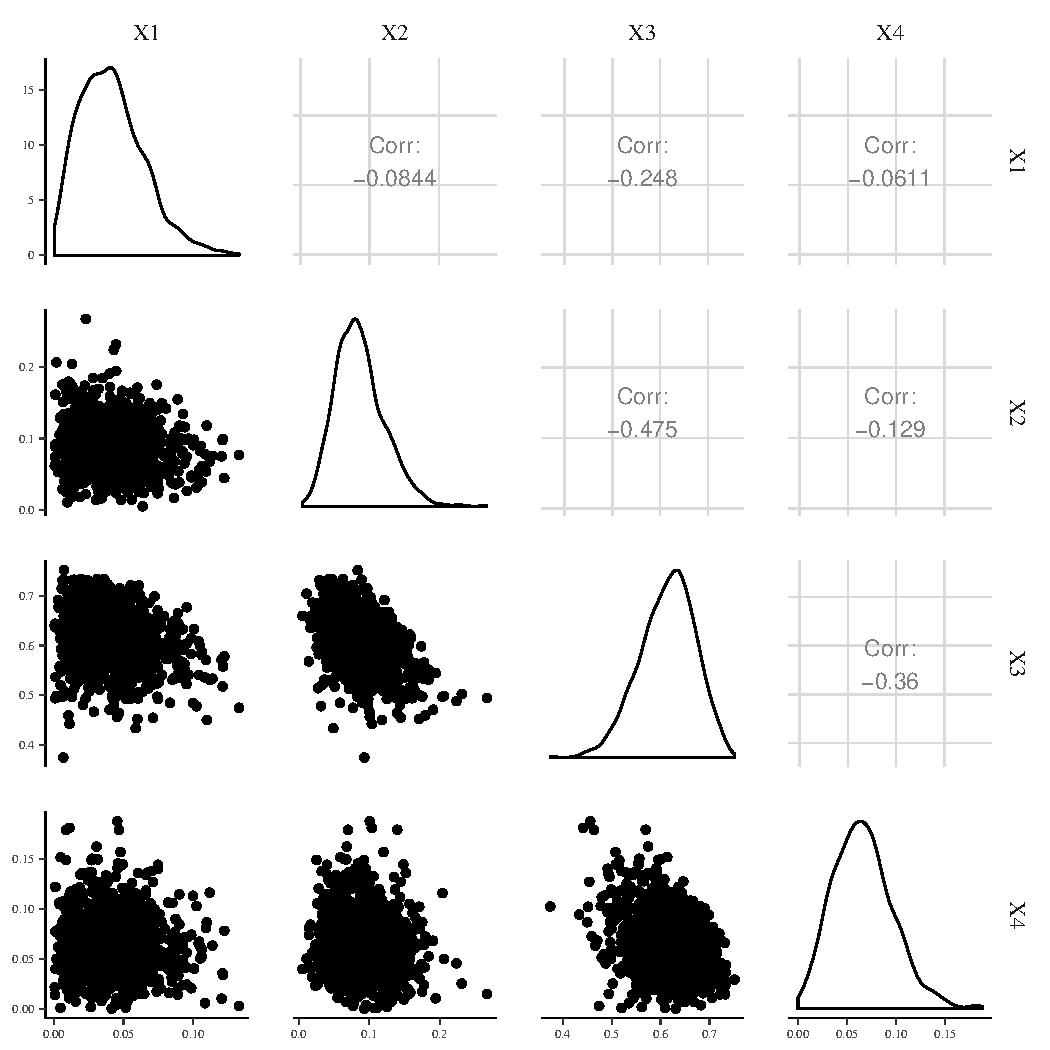
\includegraphics[width=\textwidth-3cm]{figure/ch03_figsimdata_LMG_plot-1} 

}

\caption[LMG distributions of the predictors]{LMG distributions of the predictors.}\label{fig:simdata.LMG.plot}
\end{figure}


\end{knitrout}

\begin{table}[h]
\caption{Variance decomposition for non-stochastic predictors. I~=~LMG~values, J~=~joint~contribution, Total~=~total explained variance in one-predictor model.}
\centering
\begin{tabular}{clll}
  \toprule
  \multicolumn{1}{c}{\textbf{Variable}} & \multicolumn{1}{c}{\textbf{I}} &\multicolumn{1}{c}{\textbf{J}} & \multicolumn{1}{c}{\textbf{Total}} \\
  \hline
x1 & 0.21 (0.108, 0.325)  & 0.054 (0.032, 0.076)   & 0.263 (0.149, 0.393)  \\ 
x2 & 0.15 (0.064, 0.253)  & -0.011 (-0.023, \ensuremath{3.77\times 10^{-5}})   & 0.138 (0.056, 0.239)  \\ 
x3 & 0.187 (0.09, 0.293)  & 0.037 (0.014, 0.06)   & 0.225 (0.113, 0.352)  \\ 
x4 & 0.187 (0.087, 0.304)  & 0.013 (0.005, 0.02)   & 0.2 (0.093, 0.316)  \\ 
   \bottomrule
\end{tabular}
\label{tbl:nonstochEx1}
\end{table}




\begin{table}[h]
\caption{Variance decomposition for non-stochastic predictors. I~=~LMG~values, J~=~joint~contribution, Total~=~total explained variance in one-predictor only model.}
\centering
\begin{tabular}{cll}
   \toprule
   &\multicolumn{2}{c}{\textbf{LMG value (95\%-CI)}} \\
 \textbf{Variable} & \multicolumn{1}{c}{Relaimpo} & \textbf{Bayesian framework}  \\
  \hline
x1 & 0.223 (0.136, 0.334)  & 0.21 (0.108, 0.325)  \\ 
x2 & 0.154 (0.072, 0.267)  & 0.15 (0.064, 0.253)   \\ 
x3 & 0.197 (0.103, 0.306)  & 0.187 (0.09, 0.293)  \\ 
x4 & 0.193 (0.101, 0.316) & 0.187 (0.087, 0.304)  \\ 
   \bottomrule
\end{tabular}
\label{tbl:nonstochEx1relamip}
\end{table}

\FloatBarrier


In this example, we know, that the predictor values were sampled from a normal distribution. It would therefore be more reasonable to assume stochastic predictors. Under the assumption of weak exogeinity and conditional independence, the posterior distributions of the regression parameters $\bbeta$ are valid for non-stochastic and stochastic predictors. However, the uncertainty about the LMG values needs to include the uncertainty about the covariance matrix. If we know the distribution of the predictors we can incorporate this information and obtain the posterior distribution of the covariance matrix. The package \texttt{Jags} was used for inference about the covariance matrix in a Bayesian way. The R-code of the covariance inference can be found in Appendix~\ref{r03:covminf} and the R-code to get the $\Rtwo$ values can be found in Appendix~\ref{r03:LMG.covm}. As an alternative, non-parametric bootstrap was used for inference about the covariance matrix. The R-code of the adapted LMG function can be found in Appendix~\ref{r03:LMG.boot}.

Using the bootstrap samples of the covariance matrix or samples from the posterior covariance matrix produced  very similar LMG distributions. Bootstrap seems to be a valuable option for stochastic predictors when the distribution of the predictors is unknown. Even when the distribution is known, the difference seems to be tiny. A benefit of going the full Bayesian way is that we can also include prior knowledge about the covariance matrix. Using the default priors further produced very similar LMG distribution as using the non-parametric bootstrap option of the \texttt{relaimpo} package. Table~\ref{tbl:nonstochEx1relaimpstoch} shows the LMG values of these approaches. For stochastic predictors, in contrast to non-stochastic predictors, the uncertainty about the covariance matrix is reflected in the larger credible intervals. Even when the exact regression parameters were known, there would a lot of uncertainty in the LMG values caused by the uncertainty about the covariance matrix. 








\begin{table}[h]
\caption{LMG values assuming stochastic predictors with 95\% CI.}
\centering
\begin{tabular}{clll}
   \toprule
  & \multicolumn{1}{c}{\textbf{Relaimpo}} & \multicolumn{2}{c}{\textbf{Bayesian framework}} \\ \cmidrule(r){2-2}\cmidrule(l){3-4}
 \textbf{Variable} &  & \multicolumn{1}{c}{nonparameteric bootstrap}& \multicolumn{1}{c}{covariance inference} \\
 \midrule
x1 & 0.223 (0.132, 0.33)  & 0.226 (0.103, 0.371) &  0.225 (0.095, 0.367) \\ 
x2 & 0.154 (0.065, 0.275)  & 0.138 (0.055, 0.248)  & 0.14 (0.045, 0.254) \\ 
x3 & 0.197 (0.072, 0.331)  & 0.192 (0.074, 0.323)  & 0.199 (0.093, 0.326) \\ 
x4 & 0.193 (0.076, 0.325) & 0.166 (0.058, 0.345) & 0.204 (0.083, 0.323) \\ 
   \bottomrule
\end{tabular}
\label{tbl:nonstochEx1relaimpstoch}
\end{table}







\clearpage

\section{Empirical Data}
In the following section, the Bayesian LMG implementation is applied on an empirical dataset containing test scores of pupils (N = 301) from a study by \cite{Holzinger1939} available in the R package \texttt{MBESS} \citep{MBESS}. This dataset was used in \cite{Nimon2008} to present commonality analysis, which is another variance decomposition technique. Scores from a paragraph comprehension test (paragrap) were predicted by four verbal tests:  general-information (general),  sentence-comprehension (sentence) ,  word-classification (wordc), and  word-meaning (wordm) (Table~\ref{table:hs.data}). 

The aim of the regression analysis was to determine the  association between verbal ability and paragraph comprehension.  
An overview of the data is shown in Figure~\ref{fig:empi.lmg.plot}. The regression results are shown in Table~\ref{tbl:empirical.reg}). A novice researcher may wrongly conclude, that there is little association between the "non-significant" predictors (general information and word-classification) and paragraph comprehension. Given the other predictors are already included in the model, the predictors seem not to provide  much information about the expected paragraph comprehension ability. However, it should not be concluded from this regression table, that the association between any of these "non-significant" predictors and the dependent variable is unimportant. As shown in Figure~\ref{fig:empi.lmg.plot}, the correlations between the predictors are rather high. The LMG metric may therefore provide new information about the importance of each predictor. 

The Bayesian regression model was fitted in \texttt{rstanarm}. The default priors were used for the regression coefficients and the $\sigma^2$ parameter. A burn-in period of 20000, a sample size of 20000, and a thinning of 20 resulted in a posterior sample size of 1000. The first few posterior samples are shown in Table~\ref{tab:empirical.data.postsample2}. The resulting $\Rtwo$ of these posterior samples are shown in Table~\ref{tab:empirical.data.postsample3}. The LMG values were calculated by using \texttt{hier.part}. The  independent component (I), joint contribution (J), and total explained variance in a one-predictor model (T) are shown in Table~\ref{tbl:empirical.ijt}. Sentence-comprehension and word-meaning seem to be the most important predictors by applying the LMG metric. However, none of the predictors seem to be unimportant.  The joint contributions of each predictor were quite large.

For comparison purposes, the LMG metric was additionally calculated with the \texttt{relaimpo} package using parametric bootstrapping. The confidence intervals of  \texttt{relaimpo} were almost identical to the credible intervals of the Bayesian framework (Table~\ref{tbl:empirical.relaimp.comp}). Assuming stochastic or non-stochastic predictors resulted also in almost identical uncertainty estimates with such a large sample size (Table\ref{tbl:empirical.relaimp.comp.stoch}). 







\begin{table}
\centering
\caption{Variable description of empirical data set}
\begin{tabular}{l l}
  \toprule			
  Variable Name & Description  \\   \midrule  
  paragrap & scores on paragraph comprehension test  \\
  general & scores on general information test \\
  sentence & scores on sentence completion test\\
  wordc & scores on word classification test \\
  wordm & scores on word meaning test \\
  \bottomrule  
\end{tabular}
\label{table:hs.data}
\end{table}

\begin{figure}

{\centering 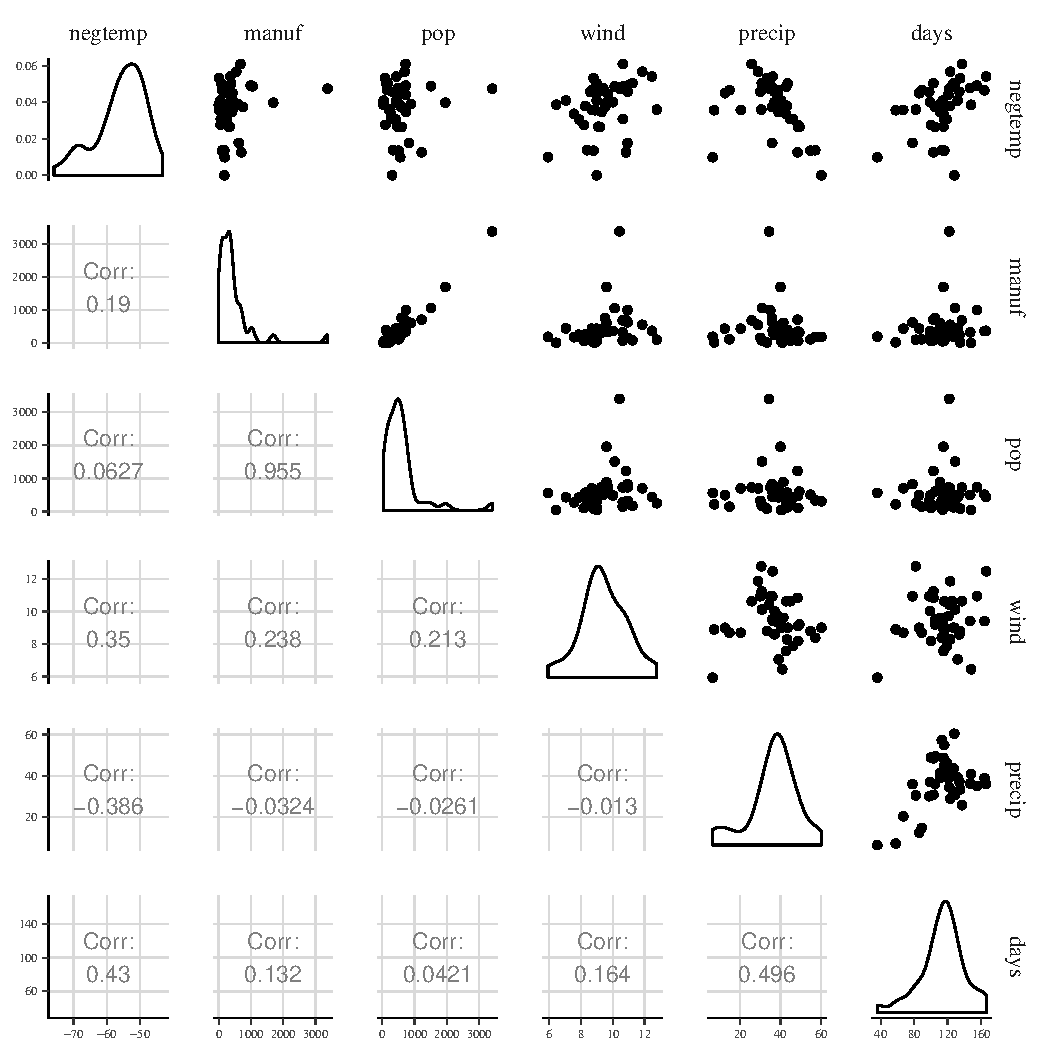
\includegraphics[width=\textwidth-3cm]{figure/ch03_figunnamed-chunk-1-1} 

}

\caption[Test scores from Holzinger and Swineford's  (1939) Study]{Test scores from Holzinger and Swineford's  (1939) Study. N=301.}\label{fig:unnamed-chunk-1}
\end{figure}






% latex table generated in R 3.4.3 by xtable 1.8-2 package
% Fri Aug 10 22:49:28 2018
\begin{table}[!h]
\centering
\caption{Regression of paragraph comprehension on verbal tests.} 
\label{tbl:empirical.reg}
\begingroup\footnotesize
\begin{tabular}{rrrr}
  \hline
 & Coefficient & 95\%-confidence interval & $p$-value \\ 
  \hline
Intercept & 0.071 & from -1.17 to 1.31 & 0.91 \\ 
  general & 0.03 & from -0.00 to 0.06 & 0.084 \\ 
  sentence & 0.26 & from 0.18 to 0.34 & $<$ 0.0001 \\ 
  wordc & 0.047 & from -0.01 to 0.11 & 0.14 \\ 
  wordm & 0.14 & from 0.08 to 0.19 & $<$ 0.0001 \\ 
   \hline
\end{tabular}
\endgroup
\end{table}


\begin{knitrout}
\definecolor{shadecolor}{rgb}{0.98, 0.98, 0.98}\color{fgcolor}\begin{table}

\caption{\label{tab:empirical.data.postsample2}Samples from the posterior distributions of the regression parameters.}
\centering
\begin{tabular}[t]{lrrrrr}
\toprule
  & general & sentence & wordc & wordm & sigma\\
\midrule
sample 1 & 0.015 & 0.312 & -0.010 & 0.159 & 2.07\\
sample 2 & 0.003 & 0.256 & 0.069 & 0.173 & 2.20\\
sample 3 & 0.029 & 0.308 & 0.022 & 0.179 & 2.10\\
sample 4 & 0.017 & 0.264 & 0.145 & 0.097 & 1.97\\
sample 5 & 0.051 & 0.262 & 0.008 & 0.134 & 2.05\\
sample 6 & 0.048 & 0.253 & 0.004 & 0.129 & 2.24\\
sample 7 & 0.031 & 0.339 & 0.045 & 0.117 & 2.18\\
sample 8 & 0.008 & 0.300 & 0.064 & 0.120 & 2.13\\
sample 9 & 0.047 & 0.250 & 0.007 & 0.166 & 2.08\\
sample 10 & 0.039 & 0.237 & 0.034 & 0.158 & 2.23\\
\bottomrule
\end{tabular}
\end{table}


\end{knitrout}

\begin{knitrout}
\definecolor{shadecolor}{rgb}{0.98, 0.98, 0.98}\color{fgcolor}\begin{table}

\caption{\label{tab:empirical.data.postsample3}$ \Rtwo$ for all submodels for the first six posterior samples.}
\centering
\begin{tabular}[t]{lrrrrrr}
\toprule
  & sample 1 & sample 2 & sample 3 & sample 4 & sample 5 & sample 6\\
\midrule
none & 0.000 & 0.000 & 0.000 & 0.000 & 0.000 & 0.000\\
general & 0.416 & 0.396 & 0.477 & 0.446 & 0.483 & 0.435\\
sentence & 0.568 & 0.528 & 0.601 & 0.586 & 0.559 & 0.505\\
wordc & 0.294 & 0.346 & 0.349 & 0.461 & 0.323 & 0.288\\
wordm & 0.524 & 0.514 & 0.575 & 0.482 & 0.525 & 0.475\\
general sentence & 0.590 & 0.552 & 0.639 & 0.615 & 0.611 & 0.551\\
general wordc & 0.444 & 0.455 & 0.515 & 0.553 & 0.509 & 0.458\\
general wordm & 0.550 & 0.535 & 0.611 & 0.533 & 0.579 & 0.523\\
sentence wordc & 0.570 & 0.546 & 0.610 & 0.635 & 0.567 & 0.511\\
sentence wordm & 0.636 & 0.606 & 0.684 & 0.629 & 0.631 & 0.570\\
wordc wordm & 0.546 & 0.558 & 0.609 & 0.596 & 0.558 & 0.503\\
general sentence wordc & 0.590 & 0.560 & 0.640 & 0.646 & 0.611 & 0.551\\
general sentence wordm & 0.637 & 0.607 & 0.689 & 0.635 & 0.644 & 0.582\\
general wordc wordm & 0.559 & 0.563 & 0.625 & 0.607 & 0.589 & 0.531\\
sentence wordc wordm & 0.636 & 0.613 & 0.686 & 0.663 & 0.633 & 0.571\\
all & 0.637 & 0.613 & 0.689 & 0.664 & 0.644 & 0.582\\
\bottomrule
\end{tabular}
\end{table}


\end{knitrout}



\begin{knitrout}
\definecolor{shadecolor}{rgb}{0.98, 0.98, 0.98}\color{fgcolor}\begin{figure}

{\centering 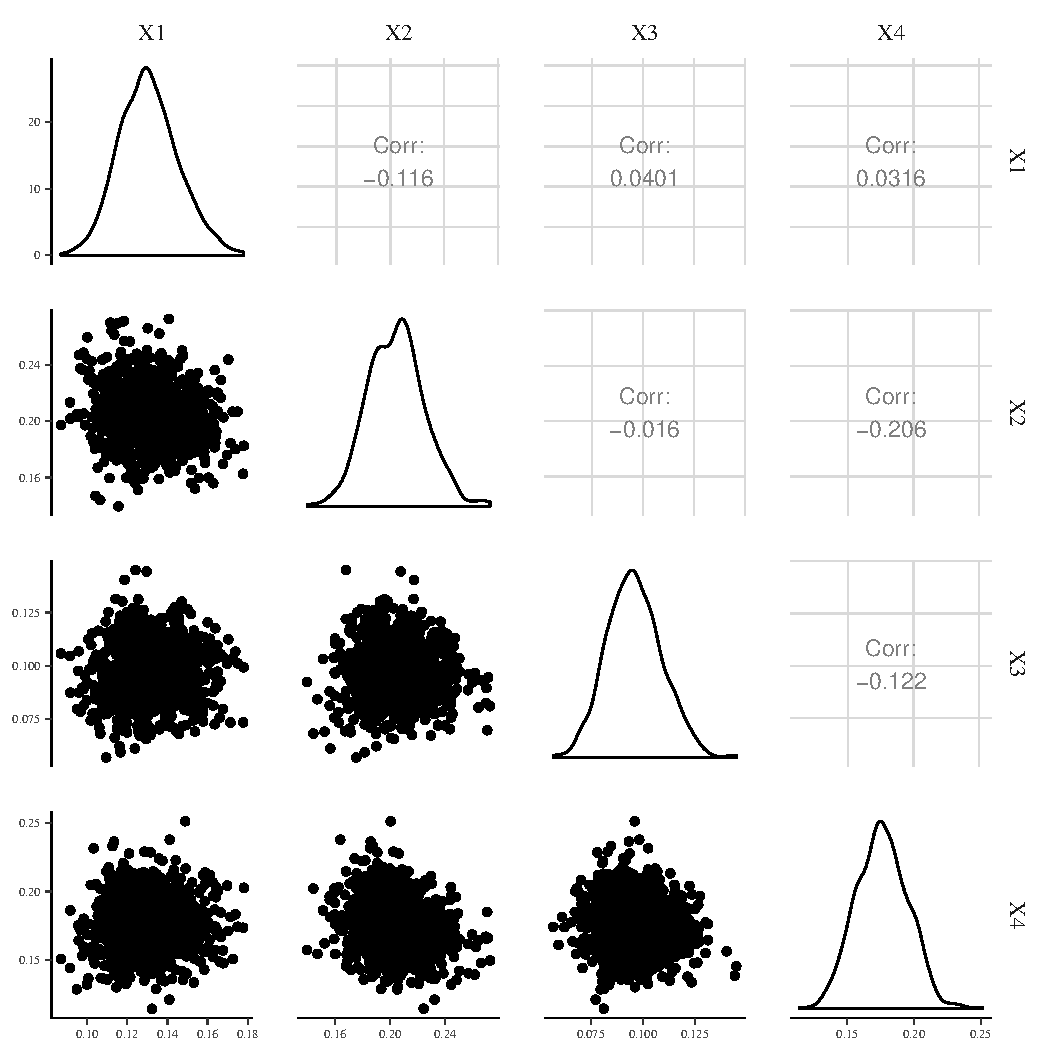
\includegraphics[width=\textwidth-3cm]{figure/ch03_figempi_lmg_plot-1} 

}

\caption[LMG distributions of the different verbal ability predictors]{LMG distributions of the different verbal ability predictors.}\label{fig:empi.lmg.plot}
\end{figure}


\end{knitrout}


\begin{table}[h]
\caption{Variance decomposition for non-stochastic predictors. I~=~LMG~values, J~=~joint~contribution, Total~=~total explained variance in one-predictor only model.}
\centering
\begin{tabular}{clll}
  \toprule
  \multicolumn{1}{c}{\textbf{Variable}} & \multicolumn{1}{c}{\textbf{I}} &\multicolumn{1}{c}{\textbf{J}} & \multicolumn{1}{c}{\textbf{Total}} \\
  \hline
general & 0.13 (0.104, 0.159)  & 0.298 (0.259, 0.332)   & 0.428 (0.363, 0.487)  \\ 
sentence & 0.203 (0.164, 0.243)  & 0.327 (0.294, 0.359)   & 0.531 (0.467, 0.594)  \\ 
wordc & 0.096 (0.072, 0.127)  & 0.24 (0.199, 0.276)   & 0.336 (0.272, 0.402)  \\ 
wordm & 0.176 (0.142, 0.215)  & 0.315 (0.284, 0.344)   & 0.493 (0.431, 0.552)  \\ 
   \bottomrule
\end{tabular}
\label{tbl:empirical.ijt}
\end{table}


\begin{table}[h]
\caption{Variance decomposition for non-stochastic predictors. I~=~LMG~values, J~=~joint~contribution, Total~=~total explained variance in one-predictor only model}
\centering
\begin{tabular}{cll}
   \toprule
   &\multicolumn{2}{c}{\textbf{LMG value (95\%-CI)}} \\
 \textbf{Variable} & \multicolumn{1}{c}{Relaimpo} & \textbf{Bayesian framework}  \\
  \hline
general & 0.131 (0.105, 0.163)  & 0.13 (0.104, 0.159)  \\ 
sentence & 0.206 (0.17, 0.248)  & 0.203 (0.164, 0.243)   \\ 
wordc & 0.096 (0.074, 0.124)  & 0.096 (0.072, 0.127)  \\ 
wordm & 0.178 (0.143, 0.219) & 0.176 (0.142, 0.215)  \\ 
   \bottomrule
\end{tabular}
\label{tbl:empirical.relaimp.comp}
\end{table}





\begin{table}[h]
\caption{Variance decomposition for stochastic predictors. I~=~LMG~values, J~=~joint~contribution, Total~=~total explained variance in one-predictor only model.}
\centering
\begin{tabular}{cll}
   \toprule
   &\multicolumn{2}{c}{\textbf{LMG value (95\%-CI)}} \\
 \textbf{Variable} & \multicolumn{1}{c}{Relaimpo} & \textbf{Bayesian framework}  \\
  \hline
general & 0.131 (0.105, 0.162)  &  0.13 (0.102, 0.161)  \\ 
sentence & 0.206 (0.168, 0.25)  &  0.204 (0.166, 0.245)   \\ 
wordc & 0.096 (0.073, 0.127)  &  0.098 (0.071, 0.131)  \\ 
wordm & 0.178 (0.145, 0.218) &  0.177 (0.14, 0.216) \\ 
   \bottomrule
\end{tabular}
\label{tbl:empirical.relaimp.comp.stoch}
\end{table}




\bibliographystyle{mywiley} 
\bibliography{biblio}
\end{document}
